
%
% Real introduction
%
The field of High Energy Physics (HEP), also known as elementary particle physics,
focuses on the study of the fundamental particles that make up the universe and their interactions via the basic forces of nature.
%
The quest for the smallest constituent of matter has its route back to the time of ancient Greece;
however, scientific attempts to understand the smallest constituent of matter started in much more recent time.
%
Particle physics emerged as a field of scientific study in the early 20th century,
when scientists began to probe the subatomic structure of matter.
%
Later, developments
of high-energy particle accelerators such as the cyclotron and the synchrotron, allowed
for the study of particles at ever-higher energies and smaller scales.
%


%
% Quarks/leptpons
%
As of now, the observed fundamental particles and their properties and interactions are thought to be described by the Standard Model (SM) of particle physics.
The SM includes six quarks (in three generations), six leptons, four gauge bosons, and the scalar Higgs boson along with antimatter particles as shown in Fig.~\ref{fig:SMParticles}.
%%
The SM of particle physics successfully describes a vast range of subatomic phenomena with outstanding precision.

\begin{figure}[t!]
\centering
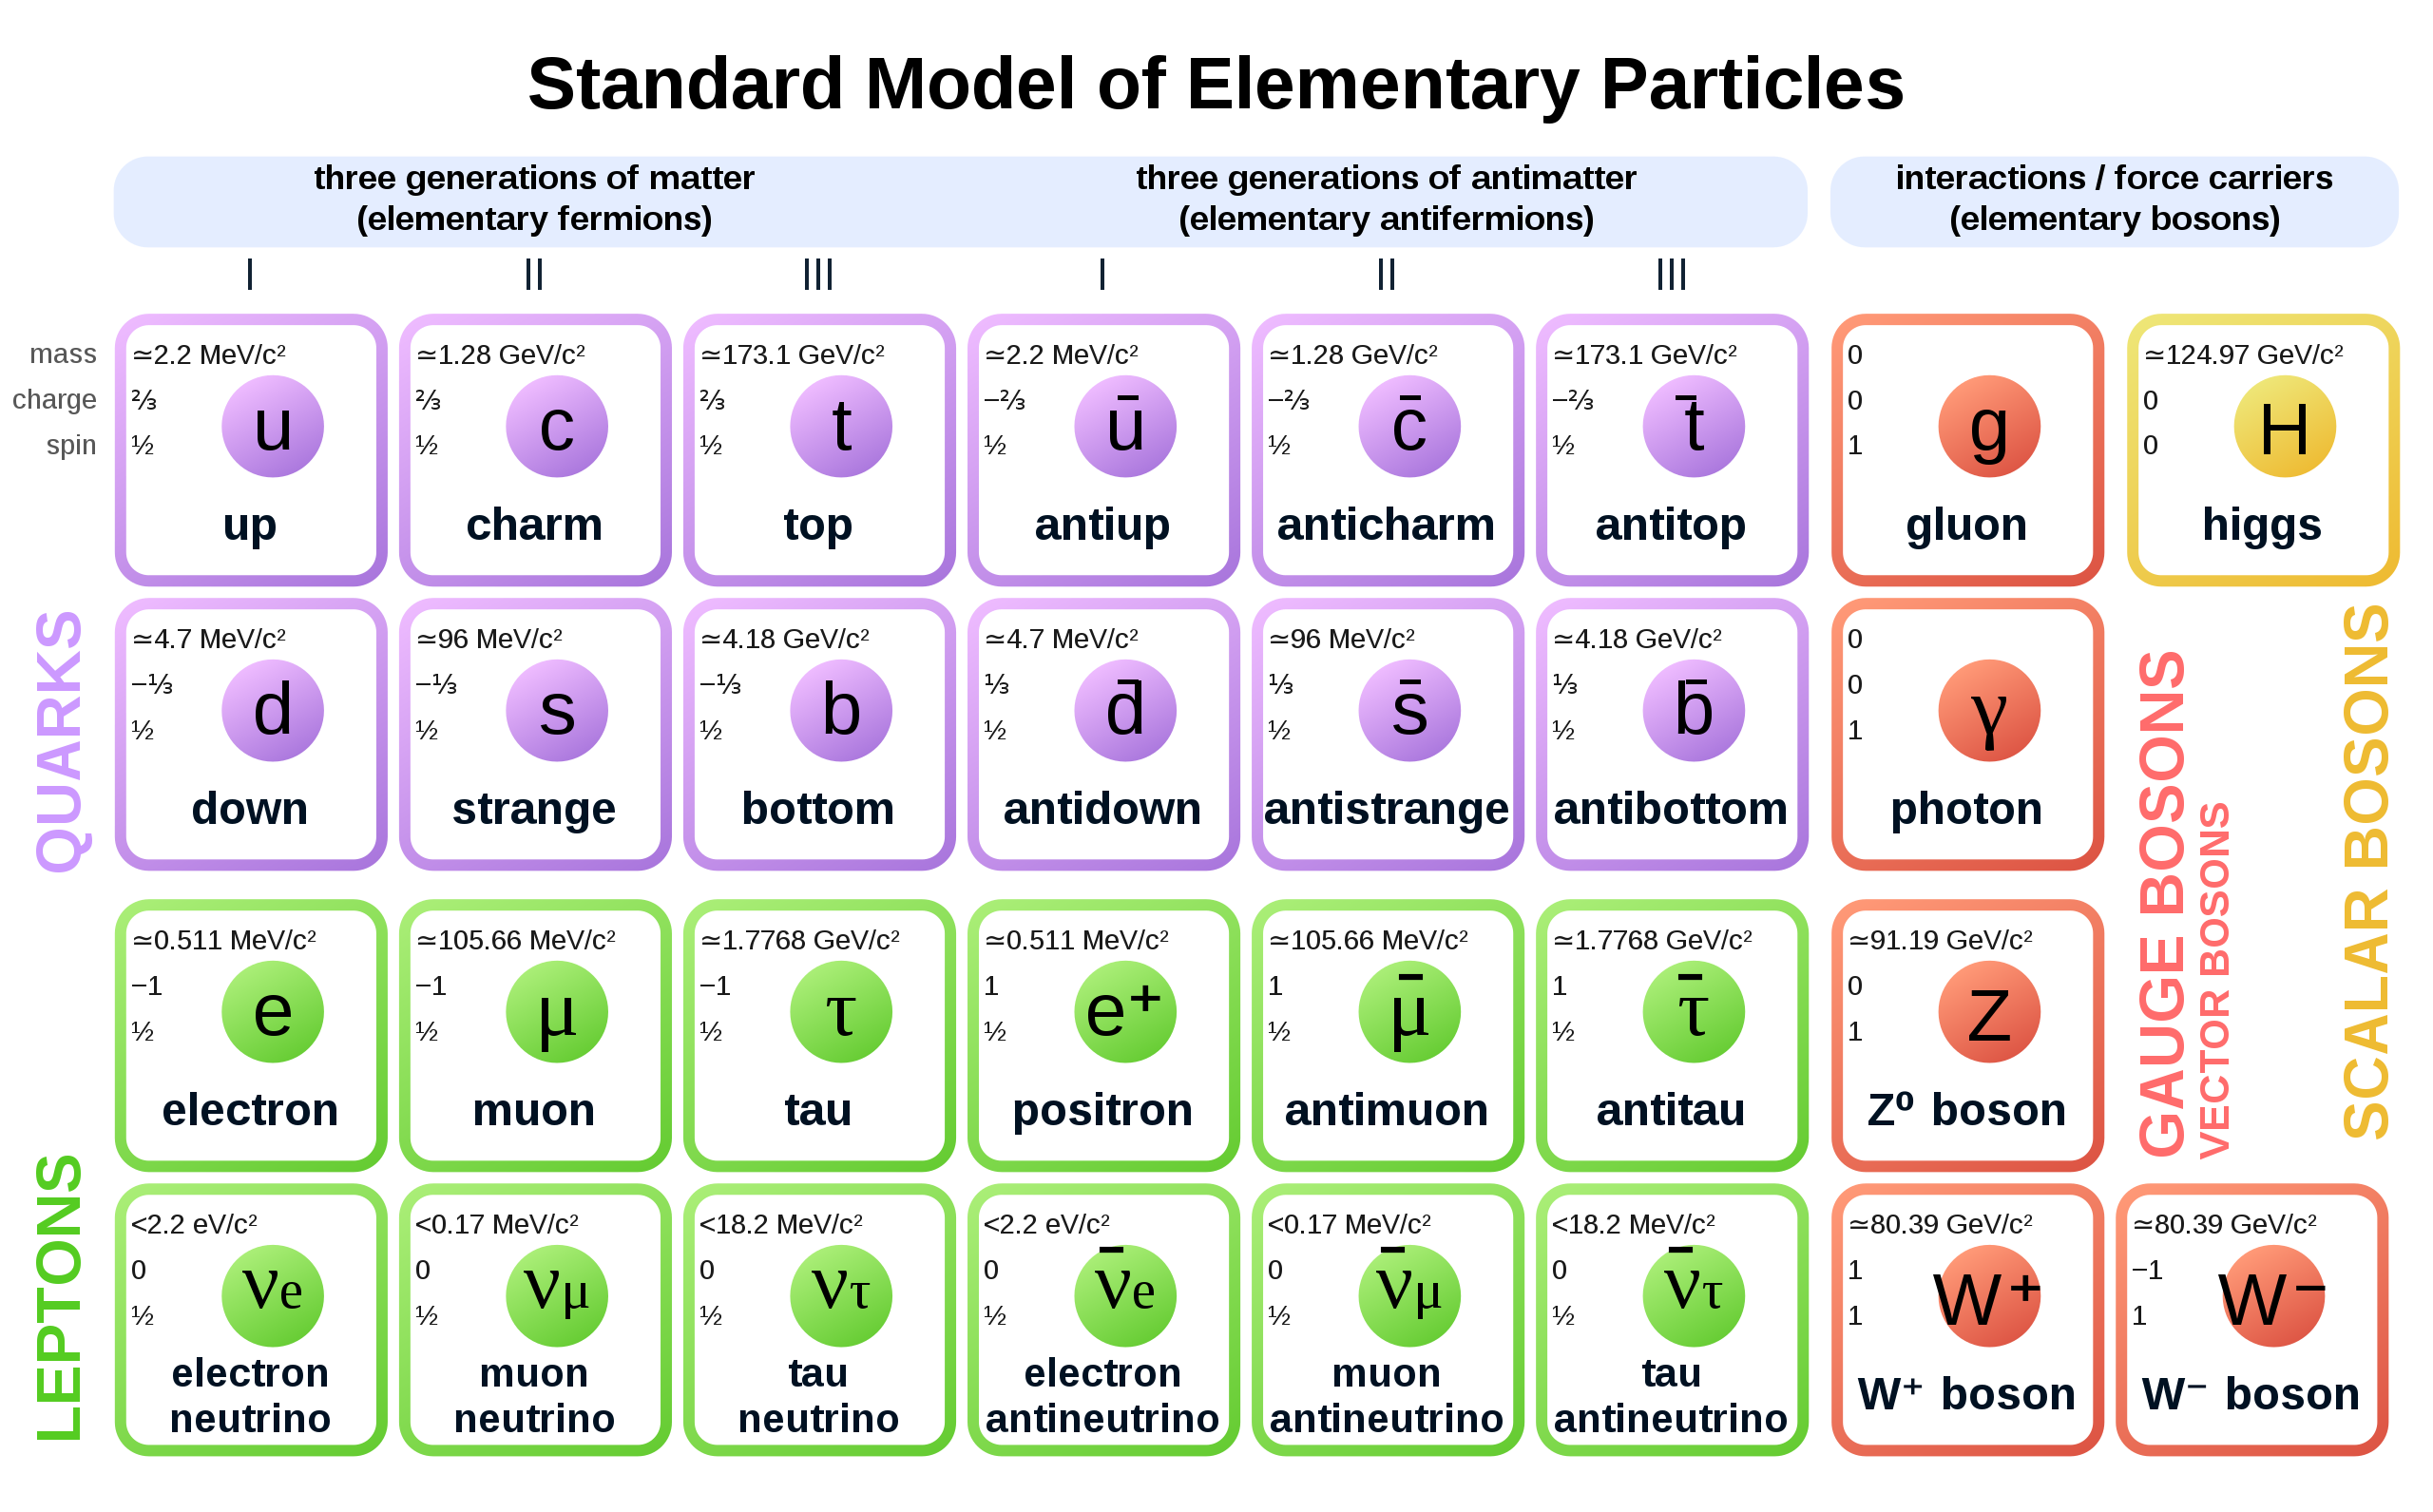
\includegraphics[width=0.99\textwidth]{figures/SMtable.png}
\caption[Summary of standard model fundamental particles]{Summary of SM fundamental particles. Figure source~\cite{SMtable}.
\label{fig:SMParticles}}
\end{figure}


%
% LHC and experiments, Very brief physics summary
%
The Hadron Collider at CERN, Geneva, Switzerland is currently the largest and highest energy particle accelerator.
The LHC consists of a 27-km ring of superconducting magnets with a number of accelerating structures to boost the energy of the particles along the way.
The LHC can acclerate different types of beams and can produce proton-proton collisions, proton-lead collisions, and lead-lead collisions; however, the main operation mode provides proton-proton collisions.
%
The first proton-proton collisions were achieved by the LHC in 2010 at an energy of 3.5 teraelectronvolts (TeV) per beam, about four times the previous world record.
Over years, the collision energy was inceased and collision rate was also increased.
As of the year of 2024, the LHC collides protons at the center-of-mass energy of $\sqrt{s}=13.6$\TeV.
%
The beams in the LHC cross each other (called bunch crossing) at four points where the ALICE, ATLAS, CMS, and LHCb detectors are located.
%
Since the start of its operation, the experiments at the LHC provide a wide range of physics results and advanced our understanding of elementary particles and their interations.
%
Among various results from LHC experiments, the most signicant one is probably the discovery of the Higgs boson by the ATLAS and CMS experiments~\cite{ATLAS:2012yve,CMS:2012qbp,CMS:2013btf}
in the mass region of around 125\GeV, announced in July, 2012.
%
Since its discovery, the Higgs boson properties have been studied in detailed in different production and decay modes by both ATLAS and CMS experiments.
In addition, all LHC experiments have been making a wide range of measurements to probe elementary particle properties and performing searches for ``new physics`` beyond the SM, and so far no result show significant discrepancies with respect to expectations from the SM.

%
%
%
For these physics studies are not possible without the high performant particle detector.
Among four major LHC experiments, I worked on the CMS experiment.
The CMS detector is described in detail in these references~\cite{CMS,CMS:2023gfb}, and some important aspects are highlighted below.

%
%
%
\section{CMS Detector}

The CMS detector is one of the general purpose detectors at the LHC.
%
Similarly to many other general purpose detectors for hadron collider experiments, the CMS detector consits of multiple subsytems:
the solenoid magnet that bents charged particles, charged particle tracking detector, electromagnetic and hadron calorimeters, and muon detectors.
% Directly taken from
% https://twiki.cern.ch/twiki/bin/viewauth/CMS/Internal/PubDetector
% Long article version.
The central feature of the CMS apparatus is a superconducting solenoid of 6\unit{m} internal diameter, providing a magnetic field of 3.8\unit{T}. Within the solenoid volume are a silicon pixel and strip tracker, a lead tungstate crystal electromagnetic calorimeter (ECAL), and a brass and scintillator hadron calorimeter (HCAL), each composed of a barrel and two endcap sections. Forward calorimeters extend the pseudorapidity coverage provided by the barrel and endcap detectors. Muons are reconstructed in gas-ionization detectors embedded in the steel flux-return yoke outside the solenoid.
The central feature of the CMS apparatus is a superconducting solenoid of 6\unit{m} internal diameter, providing a magnetic field of 3.8\unit{T}.
%
Each of these detector components is described below.

\subsection{Tracker}

What is the main purpose/function of the tracker?
What is the geometry/structure/dimension?
Possibley some purformance measures.

\subsection{Superconducting Magnet}

What is the main purpose/function of the tracker?
What is the geometry/structure/dimension?

\subsection{Electromagnetic Calorimeter}

What is the main purpose/function of the tracker?
What is the geometry/structure/dimension?
Possibley some purformance measures.

\subsection{Hadronic Calorimeter}

What is the main purpose/function of the tracker?
What is the geometry/structure/dimension?
Possibley some purformance measures.

\subsection{Muon Detector}

What is the main purpose/function of the tracker?
What is the geometry/structure/dimension?
Possibley some purformance measures.

%Here is the introduction to the topic.
%When chapters are referenced, the graduate school requires that words are used rather than numbers, e.g. ``Chapter One'' should be used instead of ``Chapter 1.''
%Use the command \verb|\cref| to reference chapters, for example \verb|\cref{chapter:ch1}|.
%The outline is as follows.
%\cref{chapter:ch2} is about paragraphs and sections.
%\cref{chapter:ch3} discusses footnotes and citations.
%\cref{chapter:ch4} presents floats.
%\cref{chapter:ch5} talks about lists.
%\cref{chapter:ch6} is the conclusion.
